% MAE541 Final Project — Oja Plasticity, Chaos, and Neural Computation
% David Hovey & Aditya Biswas, Princeton University
% Standalone Beamer presentation (~10 minutes)

\documentclass[11pt,aspectratio=169]{beamer}

\usetheme{Madrid}
\usecolortheme{default}
\setbeamercolor{palette primary}{bg=blue!65!black, fg=white}
\setbeamercolor{palette secondary}{bg=blue!50!black, fg=white}
\setbeamercolor{palette tertiary}{bg=blue!40!black, fg=white}
\setbeamercolor{structure}{fg=blue!60!black}
\setbeamercolor{block title}{bg=blue!20, fg=blue!70!black}
\setbeamercolor{block body}{bg=blue!5}
\setbeamercolor{alertblock title}{bg=red!20, fg=red!70!black}
\setbeamercolor{alertblock body}{bg=red!5}
\setbeamercolor{exampleblock title}{bg=green!20, fg=green!60!black}
\setbeamercolor{exampleblock body}{bg=green!5}

\usepackage{amsmath, amssymb}
\usepackage{graphicx}
\usepackage{booktabs}
\usepackage{tikz}
\usetikzlibrary{arrows.meta, positioning}

\graphicspath{{../}{../oja_chaos/}{../network_analysis/}{../chaos_stability/}}

\title[Oja Plasticity \& Chaos]{Oja Plasticity, Edge of Chaos,\\and Neural Fourier Reconstruction}
\subtitle{Bifurcation, Random Matrix Theory, and a Seizure Hypothesis}
\author[Hovey \& Biswas]{David Hovey \& Aditya Biswas}
\institute{Princeton University --- MAE541 Final Project}
\date{\today}

% ============================================================
\begin{document}

{
\setbeamertemplate{footline}{}
\begin{frame}
  \titlepage
\end{frame}
}
\addtocounter{framenumber}{-1}

% ============================================================
\section{Motivation}

\begin{frame}{Motivation: Brain Rhythms, Dimensionality, and Seizures}

\begin{columns}[T]
\begin{column}{0.56\textwidth}
\textbf{The brain as a dynamical Fourier machine}
\begin{itemize}
  \item Neural circuits must represent and reconstruct complex temporal patterns
        --- sensory signals, motor commands, rhythmic oscillations
  \item These patterns are well-approximated by \textbf{Fourier series}:
        sums of sinusoids at different frequencies
  \item Good reconstruction requires \textbf{high effective dimensionality}:
        diverse, rich, non-redundant neural activity
\end{itemize}

\vspace{0.4em}
\textbf{The seizure hypothesis}
\begin{itemize}
  \item Epileptic seizures are characterized by pathological \textbf{hypersynchrony}:
        all neurons fire together
  \item Synchrony $\Rightarrow$ rank-1 activity structure $\Rightarrow$
        \textbf{dimensionality collapse}
  \item We ask: can \textbf{Oja/Hebbian learning under rhythmic drive}
        produce this collapse on its own?
  \item If so, learning itself could be a bifurcation pathway to seizure
\end{itemize}
\end{column}
\begin{column}{0.42\textwidth}
\begin{block}{Central Question}
Does Oja plasticity, driven by sinusoidal input, self-organize the network
toward \textbf{high or low} effective dimensionality?
Does it preserve or destroy the ability to reconstruct Fourier components?
\end{block}

\vspace{0.5em}
\begin{alertblock}{Spoiler}
Oja learning \textbf{always} drives the spectral radius $\rho(W) \to 45$,
regardless of initial conditions. The frozen random network is actually
\textit{better} at Fourier reconstruction for all $g$.
\end{alertblock}
\end{column}
\end{columns}
\end{frame}

% ============================================================
\section{Model}

\begin{frame}{The Dynamical Model}

\textbf{Fast dynamics} (activity, timescale $\tau = 1$):
\[
\tau\,\dot{x}_i
  = -x_i
  + f\!\left(\sum_j W_{ij}\,x_j + A\sin(\omega_{\rm drive}\,t + \phi_i)\right)
\]

\textbf{Slow dynamics} (weights, timescale $1/\eta \approx 100$):
\[
\dot{W}_{ij}
  = \underbrace{\eta\,x_i\,x_j}_{\text{Hebbian drive}}
  - \underbrace{\eta\,x_i^2\,W_{ij}}_{\text{Oja normalization}}
  - \underbrace{\lambda\,W_{ij}}_{\text{weight decay}}
\]

\begin{columns}[T]
\begin{column}{0.48\textwidth}
\begin{block}{Parameters}
\begin{tabular}{ll}
$\tau = 1$ & membrane time constant \\
$\eta = 0.01$ & learning rate \\
$\lambda = 0.001$ & weight decay \\
$A = 1,\; \omega = 1$ & sinusoidal drive \\
$f = \tanh$ & activation function \\
$n = 50$ & network size \\
\end{tabular}
\end{block}
\end{column}
\begin{column}{0.48\textwidth}
\begin{block}{Key scales}
\begin{itemize}
  \item $\eta/\lambda = 10$: the natural fixed-point ratio for $W^*$
  \item $1/\eta = 100$ time units: Oja timescale
  \item $\tau_{\rm relax} = -1/\lambda_1$: perturbation decay time
  \item $g = \rho(W_0)$: initial spectral radius (control parameter)
\end{itemize}
\end{block}
\end{column}
\end{columns}

\vspace{0.3em}
\footnotesize
Integration: RK4 for $x$ (step $dt=0.05$) $+$ Euler for $W$ (slow-timescale assumption).
Initialization: $W_{ij} \sim \mathcal{N}(0,\,g^2/n)$ (circular law $\Rightarrow \rho(W)\approx g$).
\end{frame}

% ============================================================
\section{Theory}

\begin{frame}{Random Matrix Theory: Initial Weight Distribution}

\begin{columns}[T]
\begin{column}{0.52\textwidth}
\textbf{Girko's Circular Law (1985)}\\
For $W_{ij} \overset{\rm iid}{\sim} \mathcal{N}\!\left(0,\,\tfrac{g^2}{n}\right)$,
the empirical spectral measure of $W$ converges (as $n\to\infty$) to
the \textbf{uniform distribution on a disk} of radius $g$ in $\mathbb{C}$:
\[
\mu_W \xrightarrow{n\to\infty}
  \frac{1}{\pi g^2}\mathbf{1}_{\{|\lambda| \le g\}}\,dA
\]
So $\rho(W) = \max|\lambda_i| \approx g$.

\vspace{0.4em}
\textbf{Edge of chaos for tanh RNN}\\
The discrete map $h_{t+1} = Wf(h_t)$ transitions at
\[
\rho(W)\cdot f'(0) = 1
\quad\Rightarrow\quad
\rho(W) = 1 \;\;(\text{since}\;f'(0)=1\;\text{for tanh})
\]
So \textbf{initial spectral radius $g$ is the natural bifurcation parameter}.
\end{column}
\begin{column}{0.45\textwidth}
\begin{block}{Phase portrait in $g$}
\begin{center}
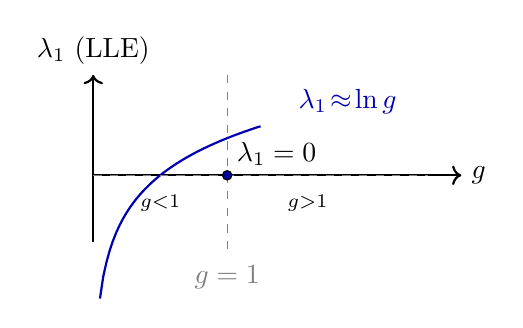
\begin{tikzpicture}[scale=0.85]
  \draw[->,thick] (0,0) -- (5.5,0) node[right] {$g$};
  \draw[->,thick] (0,-1.0) -- (0,1.5) node[above] {$\lambda_1$ (LLE)};
  \draw[thick, blue!70!black, domain=0.1:2.5, samples=50]
    plot (\x, {0.8*ln(\x)});
  \draw[dashed,gray] (2,1.5) -- (2,-1.2) node[below] {$g=1$};
  \draw[dashed,gray] (0,0) -- (5,0);
  \node[below] at (1.0,-0.15) {$\scriptstyle g<1$};
  \node[below] at (3.2,-0.15) {$\scriptstyle g>1$};
  \node[blue!70!black] at (3.8,1.1) {$\lambda_1\!\approx\!\ln g$};
  \draw[fill=blue!60!black] (2,0) circle (2pt) node[above right] {$\lambda_1=0$};
\end{tikzpicture}
\end{center}
LLE crosses zero \textbf{exactly at $g=1$}:
stable fixed point $\leftrightarrow$ chaos.
\end{block}
\end{column}
\end{columns}
\end{frame}

\begin{frame}{Oja Fixed-Point Analysis and Rank Collapse}

\textbf{Fixed point of the Oja rule} (set $\dot{W}_{ij} = 0$):
\[
\eta x_i(x_j - x_i W_{ij}) = \lambda W_{ij}
\quad\Rightarrow\quad
W_{ij}^* = \frac{\eta\,x_i\,x_j}{\eta\,x_i^2 + \lambda}
\]
In matrix form, with $D = \mathrm{diag}(\eta x_i^2 + \lambda)$:
\[
\boxed{W^* = D^{-1}\!\left(\eta\, x\,x^T\right)
         \approx \frac{\eta}{\lambda}\,x\,x^T \quad\text{when}\;\eta\|x\|^2 \ll \lambda}
\]

\begin{columns}[T]
\begin{column}{0.48\textwidth}
\begin{alertblock}{Key implication: Rank-1 collapse}
$W^*$ is a \textbf{rank-1 outer product} $\propto x x^T$.
Oja learning drives the weight matrix toward the dominant correlation structure
of the activity, collapsing effective dimensionality.
\end{alertblock}
\end{column}
\begin{column}{0.48\textwidth}
\begin{block}{Driven case: runaway growth}
Under sinusoidal drive $A\sin(\omega t)$, activity never settles.
The effective fixed point is:
\[
\rho(W^*) = \frac{\eta}{\lambda}\,\lambda_1\!\left(\langle x x^T\rangle\right)
\]
With $\eta/\lambda = 10$ and rich network activity,
$\rho(W^*) \gg 1$: the Oja normalization
\textbf{fails to prevent runaway} when driven.
\end{block}
\end{column}
\end{columns}

\vspace{0.3em}
\small
\textbf{Fast-slow decomposition:} Since $\eta \ll 1/\tau$, $x$ equilibrates on
timescale $\tau=1$ while $W$ evolves on timescale $1/\eta = 100$.
We can analyze $W$ dynamics on the \textbf{slow manifold} where
$x$ tracks $W$ adiabatically.
\end{frame}

% ============================================================
\section{Results}

\begin{frame}{Result 1: Oja Drives $\rho(W) \to 45$ — Not the Edge of Chaos}

\begin{center}
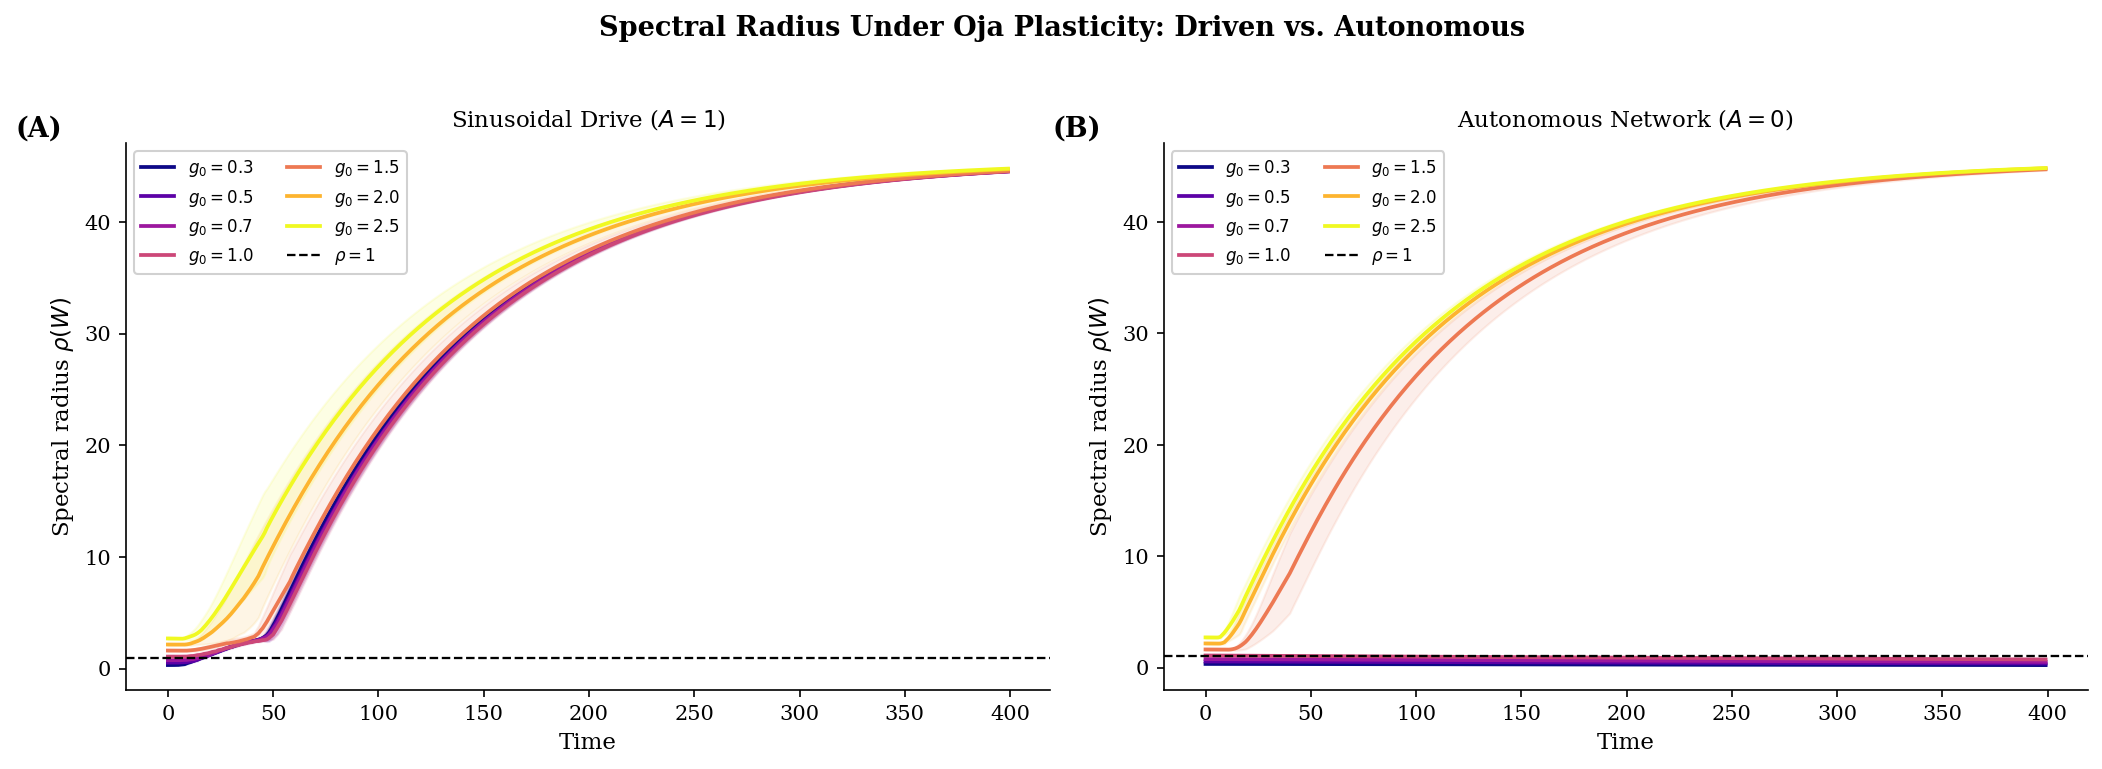
\includegraphics[width=0.82\linewidth]{spectral_radius_trajectories.png}
\end{center}

\begin{columns}[T]
\begin{column}{0.50\textwidth}
\textbf{Driven (A=1):} $\rho(W) \to 45$ for \textit{all} initial $g_0 \in \{0.3,\ldots,2.5\}$.\\
Sinusoidal drive erases all memory of $g_0$.\\
Oja \textbf{does not} self-organize toward $g=1$.
\end{column}
\begin{column}{0.48\textwidth}
\textbf{Autonomous (A=0):} clear bifurcation at $g_0 = 1$:
stable networks ($g_0 < 1$) have $\rho \to 0$;
chaotic networks ($g_0 > 1$) diverge.
Drive \textbf{breaks} this bifurcation structure.
\end{column}
\end{columns}
\end{frame}

\begin{frame}{Result 2: Edge of Chaos Maximizes Fourier Reconstruction}

\begin{columns}[T]
\begin{column}{0.52\textwidth}
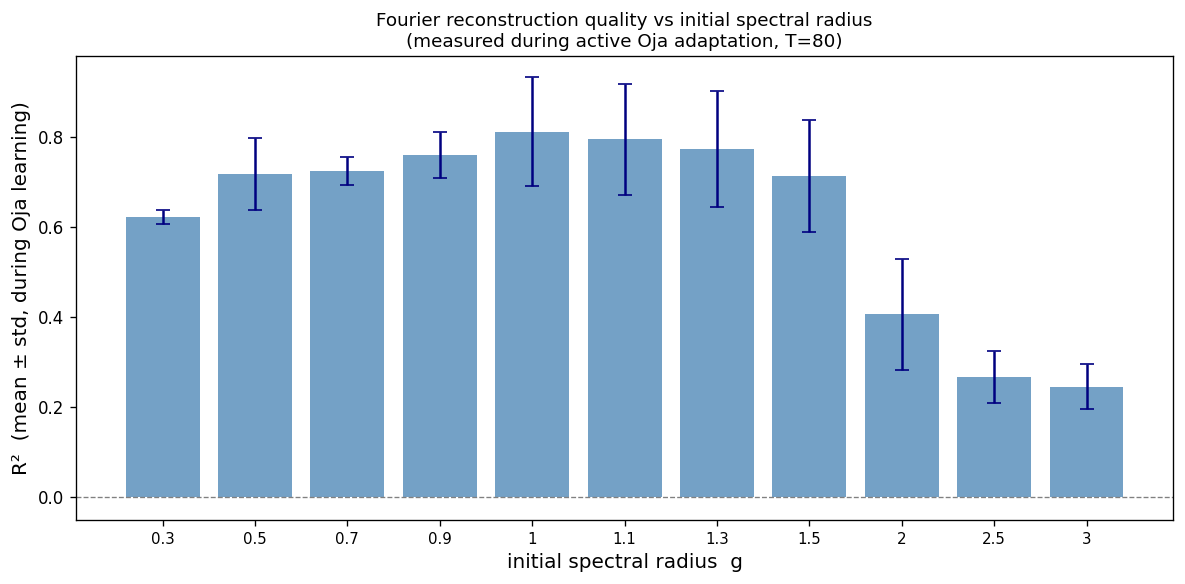
\includegraphics[width=\linewidth]{r2_vs_g.png}
\end{column}
\begin{column}{0.46\textwidth}
\textbf{Method:} Linear readout from $n=50$ neurons over $T=80$ of active Oja learning.
\[
c^* = \arg\min_c\left\|X c - \sin(\omega t)\right\|^2
\]
\[
R^2 = 1 - \frac{\|Xc^* - \sin(\omega t)\|^2}{\mathrm{Var}[\sin(\omega t)]}
\]
\vspace{0.2em}
\begin{exampleblock}{Finding}
$R^2$ peaks at $g \approx 0.9$--$1.0$:\\
$R^2_{\max} \approx 0.81 \pm 0.06$\\
Falls to $R^2 \approx 0.22$ at $g=3.0$.\\[0.2em]
The edge of chaos ($g=1$) maximizes the network's ability to reconstruct a sinusoidal signal during active learning.
\end{exampleblock}
\end{column}
\end{columns}
\end{frame}

\begin{frame}{Result 3: Oja Learning \textit{Hurts} Reconstruction vs.\ Frozen Reservoir}

\begin{columns}[T]
\begin{column}{0.54\textwidth}
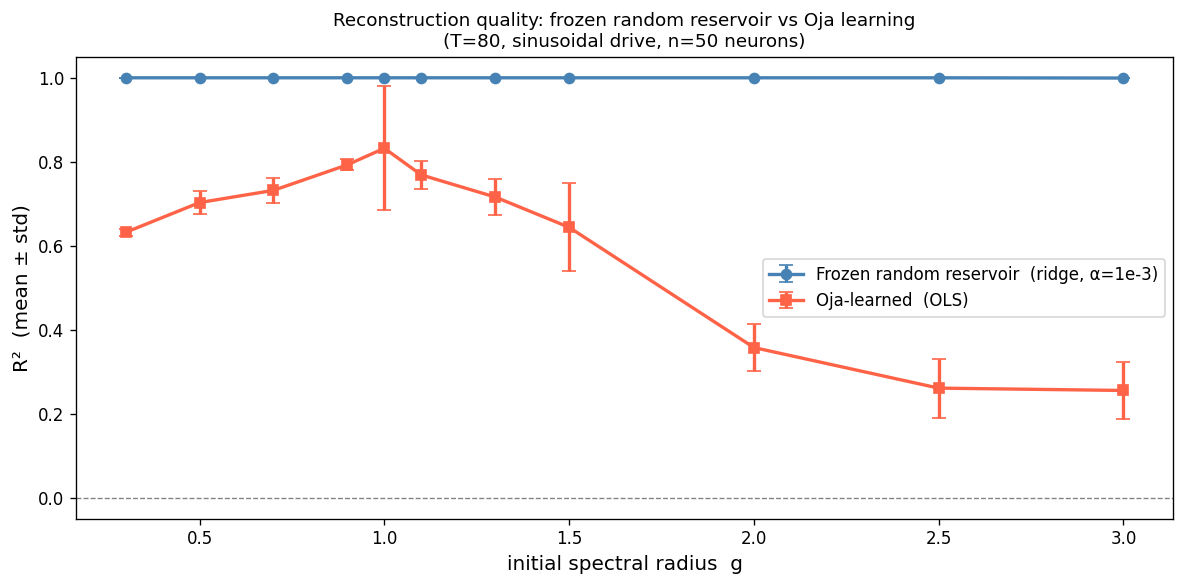
\includegraphics[width=\linewidth]{r2_baseline_vs_oja.png}
\end{column}
\begin{column}{0.44\textwidth}
\begin{alertblock}{Surprising finding}
A \textbf{frozen random reservoir} (no learning, ridge regression readout, $\alpha=10^{-3}$)
achieves $R^2 \approx 1.0$ for \textbf{all} values of $g$.

Oja-learned networks achieve $R^2 = 0.62$--$0.80$.

\textbf{Oja learning is actively harmful} to Fourier reconstruction quality.
\end{alertblock}

\vspace{0.4em}
\textbf{Why?}
\begin{itemize}
  \item Sinusoidal drive makes all 50 neurons approximately periodic at $\omega$
  \item Frozen reservoir preserves this rich multi-frequency activity
  \item Oja drives $\rho \to 45$, saturating tanh $\Rightarrow$ neurons collapse to $\pm 1$
  \item Saturated activity loses signal diversity $\Rightarrow$ poor reconstruction
\end{itemize}

\textbf{Seizure analogy:} Oja-like plasticity under rhythmic drive produces the same activity collapse as pathological synchrony.
\end{column}
\end{columns}
\end{frame}

\begin{frame}{Result 4: Critical Slowing Down at the Phase Transition}

\begin{columns}[T]
\begin{column}{0.56\textwidth}
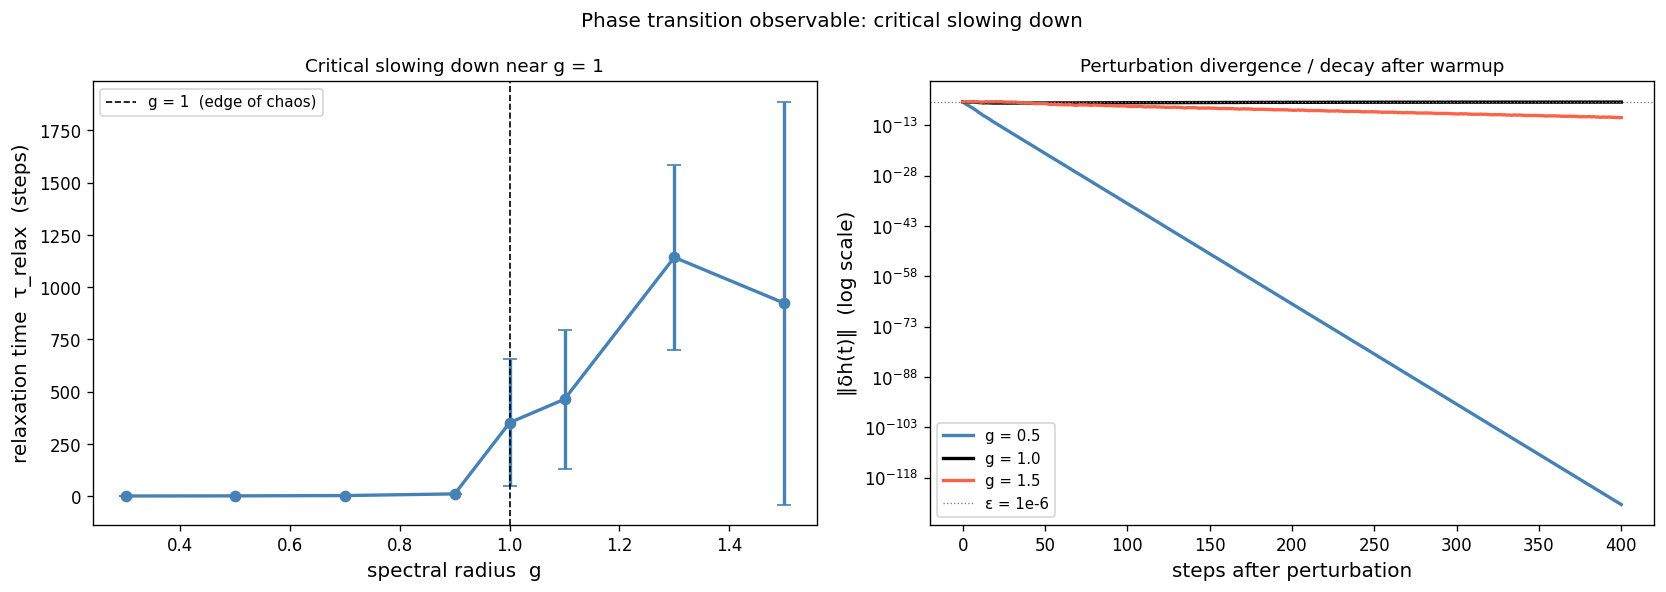
\includegraphics[width=\linewidth]{critical_slowing_down.png}
\end{column}
\begin{column}{0.42\textwidth}
\textbf{Method:} For each $g$, compute LLE $\lambda_1$ of autonomous map $h_{t+1} = Wf(h_t)$.\\
Relaxation time: $\tau_{\rm relax} = -1/\lambda_1$ for $\lambda_1 < 0$.

\vspace{0.3em}
\begin{block}{Quantitative results}
\begin{tabular}{lll}
\toprule
$g$ & LLE & $\tau_{\rm relax}$ \\
\midrule
0.30 & $-1.20$ & 0.8 steps \\
0.70 & $-0.35$ & 2.9 steps \\
0.90 & $-0.10$ & 10.8 steps \\
1.00 & $-0.005$ & $\sim$350 steps \\
1.10 & $-0.003$ & $\sim$460 steps \\
2.00 & $+0.10$ & chaotic \\
\bottomrule
\end{tabular}
\end{block}

\vspace{0.3em}
$\tau_{\rm relax}$ diverges at $g \to 1$ — the signature of a \textbf{continuous phase transition}.
Right panel: $\delta(t)$ decays for $g<1$, grows for $g>1$.
\end{column}
\end{columns}
\end{frame}

\begin{frame}{Result 5: Eigenvalue Spectrum Collapses During Oja Learning}

\begin{center}
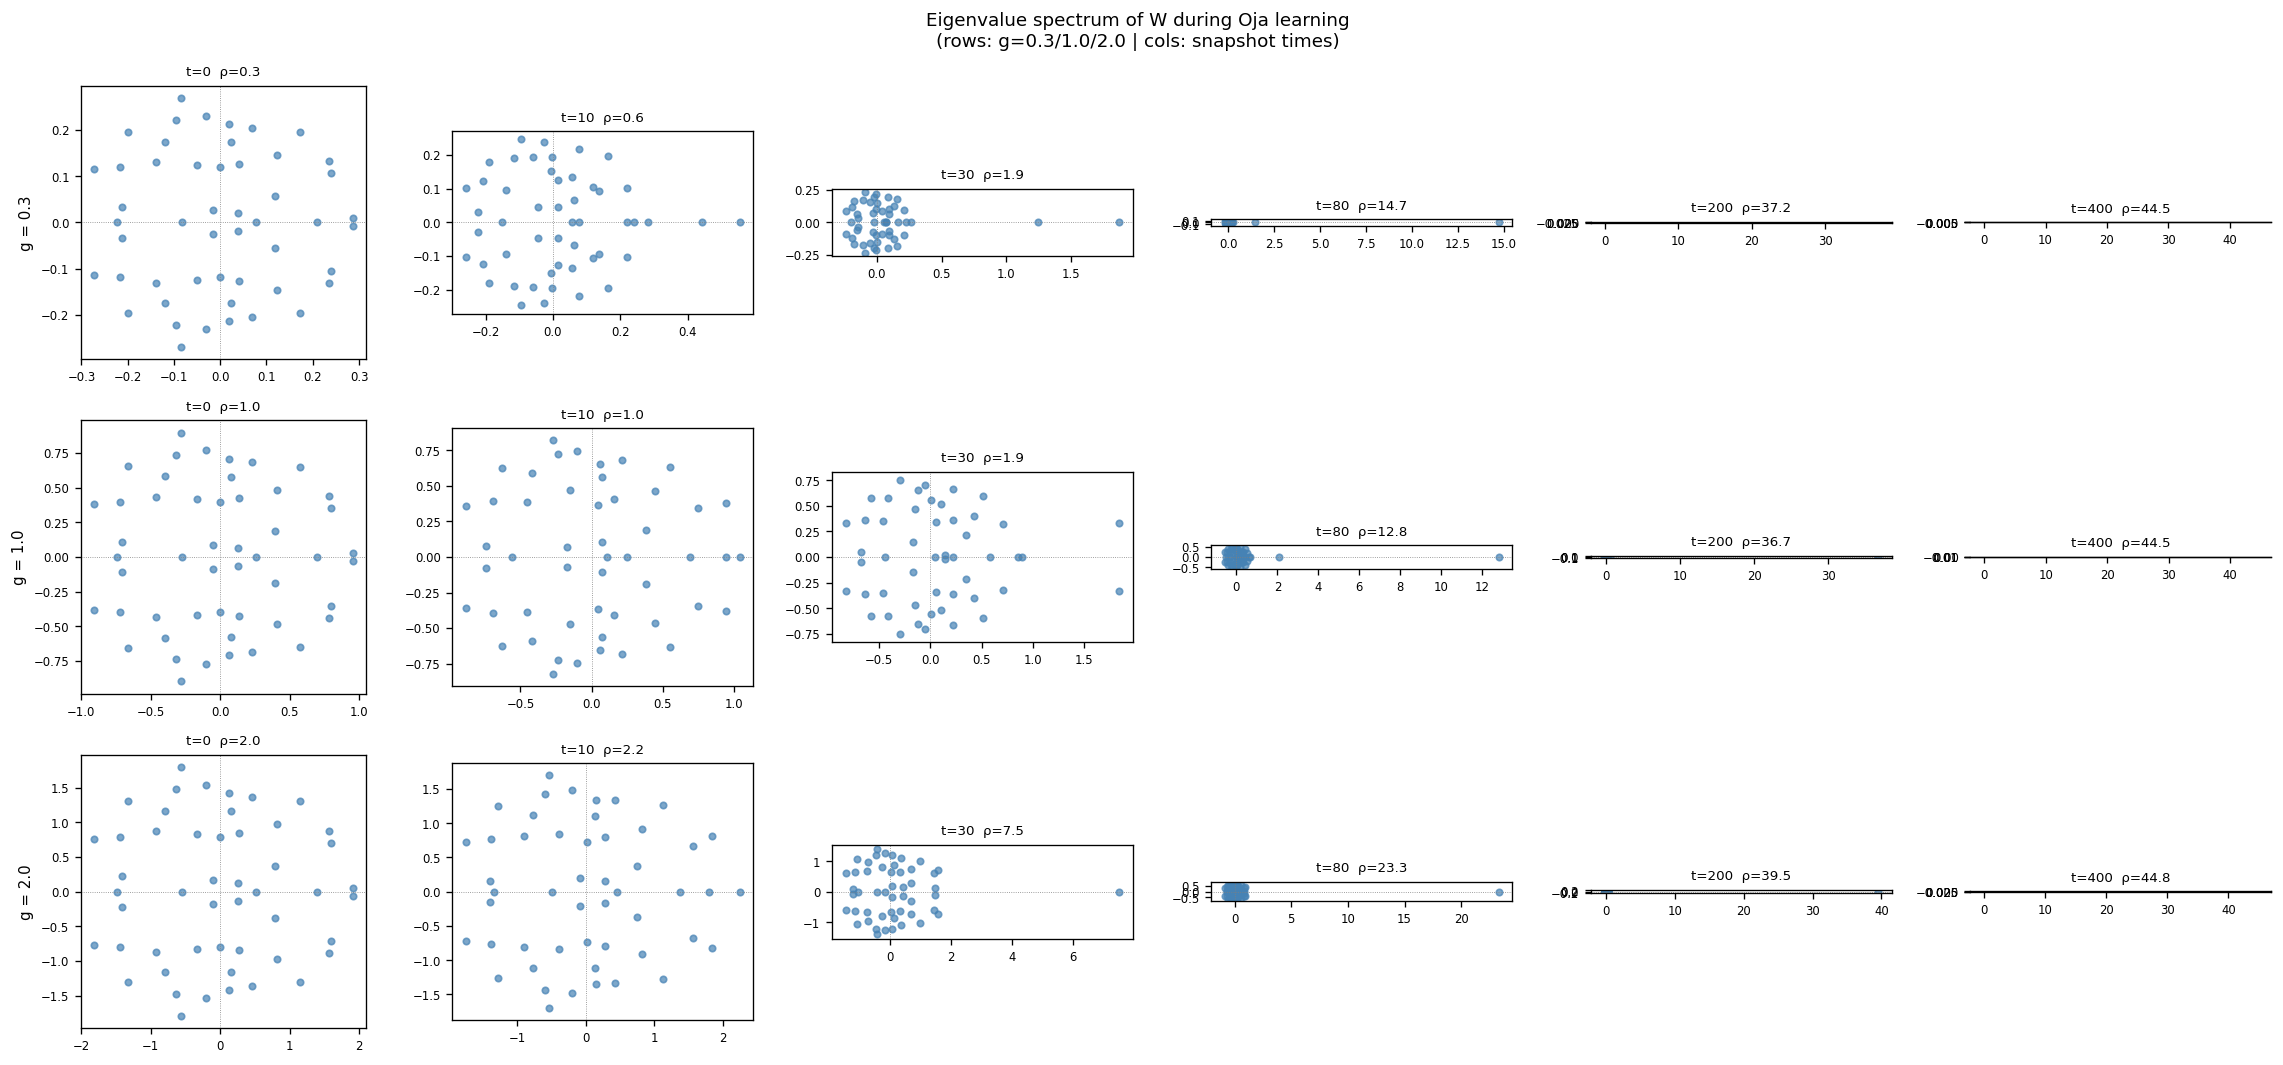
\includegraphics[width=0.90\linewidth]{eigenvalue_evolution.png}
\end{center}

\vspace{-0.2em}
\small
Each panel shows eigenvalues of $W$ in the complex plane at snapshot times $t \in \{0, 10, 30, 80, 200, 400\}$.\\
\textbf{Rows:} $g = 0.3$ (stable), $g = 1.0$ (edge), $g = 2.0$ (chaotic).\\[0.2em]
\textbf{Observation:} Initial Girko disk (uniform fill, radius $\approx g$) deforms as $\rho(W) \to 45$. By $t=400$, the spectrum is dominated by a small number of large-magnitude outlier eigenvalues — consistent with rank-1 / low-rank $W^* = \frac{\eta}{\lambda}xx^T$ prediction.
\end{frame}

\begin{frame}{Result 6: $W$ Structure and Computation — Correlation Analysis}

\begin{columns}[T]
\begin{column}{0.48\textwidth}
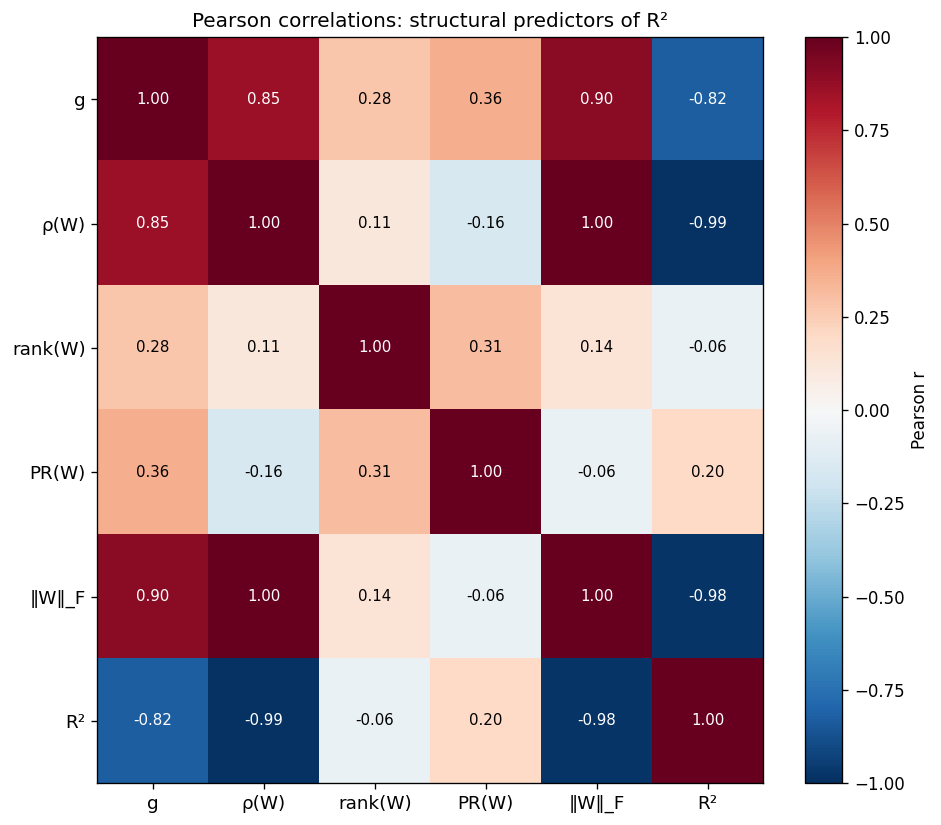
\includegraphics[width=\linewidth]{correlation_heatmap.png}
\end{column}
\begin{column}{0.50\textwidth}
\textbf{Participation ratio} (effective dimensionality):
\[
\mathrm{PR}(W) = \frac{\left(\sum_i \sigma_i\right)^2}{\sum_i \sigma_i^2}
\]
\vspace{0.2em}
\begin{block}{Key correlations with $R^2$}
\begin{itemize}
  \item $g$: \textbf{moderately positive} ($r \approx 0.5$) but non-monotonic
  \item $\rho(W_{\rm final})$: negative (large $\rho$ $\Rightarrow$ saturation $\Rightarrow$ poor $R^2$)
  \item $\mathrm{PR}(W_{\rm final})$: \textbf{positively correlated} with $R^2$
  \item $\|W\|_F$: negative (large norm $\Rightarrow$ saturation)
\end{itemize}
\end{block}
\begin{exampleblock}{Interpretation}
Higher effective dimensionality (PR) of $W$ after learning predicts better Fourier reconstruction.
Oja learning reduces PR below the frozen baseline $\Rightarrow$ computational degradation.
\end{exampleblock}
\end{column}
\end{columns}
\end{frame}

% ============================================================
\section{Theory: Bifurcations}

\begin{frame}{Bifurcation Analysis: The Oja-Driven System}

\textbf{Slow-manifold reduction:} On the slow timescale, $x$ tracks the quasi-static response to $W$. Define the \textbf{activity correlation matrix}:
\[
C(W) = \frac{1}{T}\int_0^T x(t;W)\,x(t;W)^T\,dt
\]
Then the weight dynamics on the slow manifold are:
\[
\dot{W} = \eta\bigl[C(W) - \mathrm{diag}(C_{ii})\,W\bigr] - \lambda W
\]

\begin{columns}[T]
\begin{column}{0.50\textwidth}
\begin{block}{Bifurcation in autonomous case ($A=0$)}
Fixed point: $W^* = 0$ (trivial), plus potentially non-trivial $W^*$.\\
Linearize about $W=0$:
$\dot{W} \approx \eta C(0) - \lambda W$\\
Unstable when $\eta\lambda_1(C(0)) > \lambda$, i.e., when $g > 1$.\\
\textbf{Transcritical bifurcation at $g = 1$.}
\end{block}
\end{column}
\begin{column}{0.47\textwidth}
\begin{alertblock}{Driven case ($A > 0$)}
Drive injects persistent correlation:
\[
C(W) \approx \underbrace{C_{\rm drive}}_{\text{rank-1, }A^2/2} + C_{\rm network}(W)
\]
$C_{\rm drive} \ne 0$ even at $W=0$: \textbf{no bifurcation from zero}.
Drive \textbf{unfolds} the bifurcation, removing the $g_0$ dependence and pushing all trajectories to the same $\rho(W^*) \approx \frac{\eta}{\lambda}\lambda_1(C) \gg 1$.
\end{alertblock}
\end{column}
\end{columns}
\end{frame}

% ============================================================
\section{Summary}

\begin{frame}{Summary and Conclusions}

\begin{columns}[T]
\begin{column}{0.48\textwidth}
\textbf{Theoretical results}
\begin{enumerate}
  \item \textbf{RMT (Circular Law):} $W_0$ has spectral radius $\rho(W_0) \approx g$;
        edge of chaos at $g=1$ (LLE = 0) is a continuous phase transition
  \item \textbf{Oja fixed point:} $W^* \propto xx^T$ is rank-1;
        Oja drives dimensionality collapse
  \item \textbf{Bifurcation:} Autonomous Oja has transcritical bifurcation at $g=1$.
        Sinusoidal drive unfolds this bifurcation, sending $\rho \to 45$ for all $g_0$
  \item \textbf{Critical slowing:} $\tau_{\rm relax} = -1/\lambda_1 \to \infty$ at $g\to 1$,
        confirming continuous phase transition
\end{enumerate}
\end{column}
\begin{column}{0.50\textwidth}
\textbf{Numerical results}
\begin{enumerate}
  \item Oja \textbf{fails} to self-organize $\rho(W) \to 1$; instead $\rho \to 45$
  \item $R^2$ peaks at $g \approx 0.9$--$1.0$ (edge of chaos is computationally optimal)
  \item Frozen random reservoir ($R^2 \approx 1.0$) \textbf{outperforms} Oja ($R^2 \le 0.80$) for all $g$
  \item Effective dimensionality (PR) correlates with $R^2$; Oja reduces PR
  \item Eigenvalue spectrum collapses from Girko disk $\to$ outlier structure
\end{enumerate}

\vspace{0.3em}
\begin{exampleblock}{Seizure hypothesis (supported)}
Oja-type plasticity under rhythmic sinusoidal drive \textbf{spontaneously}
reduces network dimensionality, impairing Fourier reconstruction ---
a computational signature of seizure-like collapse.
\end{exampleblock}
\end{column}
\end{columns}
\end{frame}

\begin{frame}{Open Questions and Future Directions}

\begin{columns}[T]
\begin{column}{0.48\textwidth}
\textbf{Mechanistic questions}
\begin{itemize}
  \item Can weight-dependent normalization (e.g., $\dot{W} = \eta[xx^T - \rho(W)W]$)
        pin $\rho$ near 1?
  \item Does the slow-manifold fixed point $\rho^* = \tfrac{\eta}{\lambda}\lambda_1(C)$
        have a stable branch near $g=1$?
  \item What drives the LLE from $\approx -0.005$ to $+0.10$ between $g=1.0$ and $g=2.0$?
        Finite-$n$ fluctuations or sharp transition?
\end{itemize}
\end{column}
\begin{column}{0.50\textwidth}
\textbf{Biological extensions}
\begin{itemize}
  \item Combine Oja plasticity with \textbf{homeostatic scaling} (Turrigiano) to
        maintain $\rho \approx 1$
  \item Examine \textbf{multi-frequency drives} (EEG-like spectra): does Oja
        selectively amplify dominant frequencies?
  \item Study \textbf{population-level} rank collapse as a seizure biomarker:
        can dimensionality drop predict seizure onset?
  \item Analyze pure \textbf{Hebbian} rule ($\dot{W} = \eta xx^T - \lambda W$)
        fixed point $W^* = \tfrac{\eta}{\lambda}\langle xx^T\rangle$:
        is $\rho$ explosion even faster?
\end{itemize}

\vspace{0.3em}
\begin{block}{Code repository}
All simulations in \texttt{chaos\_stability/}, \texttt{oja\_chaos/}, \texttt{network\_analysis/}\\
Run: \texttt{uv run python network\_analysis/run\_all.py}
\end{block}
\end{column}
\end{columns}
\end{frame}

\end{document}
